\newcommand \beq{\begin{eqnarray}}
\newcommand \eeq{\end{eqnarray}}
\newcommand \bea{\begin{eqnarray}}
\newcommand \eea{\end{eqnarray}}
\newcommand \avec{{\bf a}}
\newcommand \kvec{{\bf k}}
\newcommand \lvec{{\bf l}}
\newcommand \qvec{{\bf q}}
\newcommand \pvec{{\bf p}}
\newcommand \hvec{{\bf h}}
\newcommand \nvec{{\bf n}}
\newcommand \xvec{{\bf x}}
\newcommand\rvec{{\bf r}}
\newcommand\yvec{{\bf y}}
\newcommand\Rvec{{\bf R}}
\newcommand\Pvec{{\bf P}}
\newcommand\Qvec{{\bf Q}}
\newcommand\Gvec{{\bf G}}
\newcommand\Kvec{{\bf K}}
\def\simge{\mathrel{%
       \rlap{\raise 0.511ex \hbox{$>$}}{\lower 0.511ex \hbox{$\sim$}}}}
\def\simle{\mathrel{
       \rlap{\raise 0.511ex \hbox{$<$}}{\lower 0.511ex \hbox{$\sim$}}}}

\section{Introduction}
Insulator and semiconductors are characterized by a non-vanishing {\it fundamental gap}
\cite{book}, 
defined in terms of the ground state energies of a system of fixed ions as the number of electrons is varied:
\beq
\Delta_{N_e} = E_0(N_e+1)+ E_0(N_e-1)- 2 E_0(N_e)
\label{gap}
\eeq
where $E_0(N_e)$ is the ground-state energy of an $N_e$ electron system.

Within density functional theory (DFT), it is common to interpret the eigenvalues of the
Kohn-Sham equations as excitation energies, the gap being the minimum excitation energy. However, the resulting band gap
within the local density approximation (LDA) is typically found to be too small \cite{Perdew}.
This qualitative failure can be alleviated
either by hybrid functionals or by adding corrections based on GW many-body perturbation theory,
although the precise value depends on the underlying functional and approximation scheme involved \cite{book}.
In principle, the fundamental gap can be calculated from any method for ground-state energies
based on the above formula.
High-precision methods for correlation energies as, for example, provided
by quantum Monte Carlo (QMC) \cite{rev1,rev2,rev3,Ruggeri18} or coupled cluster methods
\cite{Shepherd13,Gruber18} can be used.  
In this work, we propose a method for accurate calculations of the fundamental gap
within explicitly correlated methods and demonstrate its use with fixed-node diffusion Monte Carlo (DMC) benchmark studies on solid H$_2$,  C, and Si.

Methods based on correlated many-body wave functions
are usually applied to finite-sized systems, e.g.,
%which introduces a systematic bias for extensive systems. 
%The importance of correcting finite size error in the QMC calculation of excitations has
%been pointed out previously \cite{Williamson98,Kent98,Kent99}.
limited to supercells containing only few unit cells.
QMC calculations of single-particle excitations for adding and removing electrons 
\cite{Kent98,Kent99,Mitra15,McMinis15} crucially rely on the imposed extrapolation law
(e.g., finite-size error $\propto 1/L$ in Ref.~\cite{McMinis15} opposed to $1/L^3$ in Ref.~\cite{Mitra15}, where $L$ denotes the linear extension of the supercell). This introduces considerable uncertainty in the results.
Heuristically, single-particle excitations are expected to converge slowly for electronic systems,
inversely proportional to $L$,
due to the interaction of charges across the periodic boundaries \cite{Payne,Engel}.
Extrapolations with respect to the size of the supercells are then
essential to obtain reliable values of the gap in the thermodynamic limit.

Most of the QMC calculations 
\cite{Ceperley87,Mitas94,Williamson98,Towler2000,Kolorenc08,Ma13,Wagner14,Yu15,Zheng18,Frank19} 
have therefore addressed charge-neutral, particle-hole excitations,
where faster convergence with respect to the size of the supercell is expected.
Although the comparison with experiment is appealing \cite{rev3}, 
a later, more extended DMC study \cite{Hunt} of simple semiconductor materials
with larger supercells observed a $1/L$ dependence of the gap on the size of the supercell
for both charged single-particle and charge-neutral particle-hole excitations.
In addition, 
fixed-node energy differences are not constrained to be upper bounds for particle-hole excitations
\cite{Foulkes99} since orthogonality to the ground state cannot be strictly guaranteed.
Furthermore, all QMC calculations so far have addressed excitations at selected
symmetry points contained inside the supercell of the simulation.
The fundamental gap was then estimated indirectly by introducing 
a ``scissor operator'' \cite{Azadi2017} which assumes a rigid shift of
the underlying DFT band structure over the whole Brillouin zone.

In this work, we show that twisted boundary conditions within the grand canonical ensemble
can be used
to  determine the fundamental gap from QMC without relying on the ``scissor'' approximation.
We prove that to leading order, finite size effects due to two-body correlations are of order $1/L$,
and are related to the dielectric constant of the material. Such effects
can be understood and corrected for by using
the long wavelength properties of the electronic
structure factor. 
For that, we extend the approach described in Refs.~\cite{fse,finitesize} 
which discusses the correction
of finite size effects on the ground-state energy
based on information contained in the static correlation functions of the finite system.
Using the static structure factor from simulation, it is possible to obtain estimates of finite size corrections 
for the band gap, and its asymptotic functional form 
without the need for
explicit studies at different sizes or referring to DFT or to experimental information
external to the QMC calculation.

The chapter is organized as follows. In Sec.~\ref{sec:bg-gctabc}, we describe the main ideas behind our band-gap method based on the grand canonical ensemble. In Sec.~\ref{sec:bg-fse}, we derive finite size corrections to energy differences based on an explicit many-body wave function and exact diagrammatic relations. In Sec.~\ref{sec:bg-methods}, we describe the computational methods used to calculate the fundamental gap. In Sec.~\ref{sec:bg-results}, we show results for H$_2$, C, and Si crystals
and compare with available experimental values of the gap in Sec.~\ref{sec:bg-compare}.
Finally in Sec.~\ref{sec:bg-conclude}, we summarize general features of the method
 and outline possible extensions and applications.

\section{Grand-Canonical twist-averaged boundary condition (GCTABC)\label{sec:bg-gctabc}}

In the following, we consider $N_e$ electrons in a perfect crystal,
neglecting both zero-point and thermal motion of the ions.
A uniform background charge (depending on $N_e$) is added to assure global 
charge neutrality when adding or subtracting electrons to a charge-neutral system.
The background charge will introduce a rigid shift in the density of states. However, the fundamental gap, Eq.~(\ref{gap}), is unaffected,
because the background
charge needed when adding an electron cancels against the one needed when removing an electron.
Periodic boundary conditions of the charge densities are used to eliminate surface effects.

The energetic cost of adding an electron to the system at fixed volume, $V=L^3$, defines the
chemical potential:
\beq
\mu_{N_e}^+= E_0(N_e+1)-E_0(N_e).
\eeq
A non-vanishing gap implies a discontinuity in the chemical potential from Eq.~(\ref{gap}).

It is convenient to work in the grand-canonical ensemble. There, the
chemical potential $\mu$ is treated as an independent variable and we minimize $E_0(N_e)-\mu N_e$ with respect to $N_e$ at zero temperature and fixed volume. Insulators then represent an incompressible electronic state; for values of $\mu$
within the gap, $\partial N_e/\partial \mu=0$.

To reduce finite size effects, we employ twisted boundary conditions on the many-body wave function.
As an electron is moved across the supercell, e.g., by moving an electron a distance equal to the size of the box in the $x$ direction,
\beq
\Psi (\rvec_1+L_x\hat{x}) = e^{i\theta_x} \Psi(\rvec_1),
\eeq
the phase of the many-body wave function changes by $\theta$.
The ground-state energy then depends on the twist angle, $E_0(N_e,\theta)$. 
Twist averaging
can significantly accelerate convergence 
to the thermodynamic limit \cite{Lin01}.
Within the grand-canonical ensemble \cite{fse,finitesize}, the optimal number
of electrons ${\bar N}_e(\theta)$ will depend  on $\theta$ for given chemical potential $\mu$. To fix nomenclature, we define the
\emph{mean electronic density},
\begin{equation} \label{eq:ne}
n_e(\mu)=(M_\theta V)^{-1}\sum_\theta  {\bar N}_e(\theta),
\end{equation}
and the \emph{ground-state energy density},
\begin{equation} \label{eq:e0}
e_0(\mu)=(M_\theta V)^{-1} \sum_\theta E_0({\bar N}_e(\theta),\theta).
\end{equation}
$n_e$ is determined by minimizing the free-energy density,
\begin{equation}
f=\frac{1}{M_\theta V} \sum_\theta \min_{N_e} \left[ E_0(N_e,\theta) - \mu N_e \right],
\end{equation}
where the sum is over a uniform grid containing $M_\theta$ twist angles.
For any single-electron theory, the electronic density $n_e(\mu)$
and the ground-state energy density $e_0(\mu)$ coincide exactly with the corresponding
thermodynamic limit values for a sufficiently large value of $M_\theta$, e.g., when the sum over twists becomes an integral over the 
Brillouin zone.  Size effects remaining after twist averaging are due to electron-electron correlations.

Figure~\ref{fig:H_C2CP250}(a) illustrates $e_0(\mu)$ and $n_e(\mu)$ for solid molecular hydrogen, computed from HSE functional and from QMC (see Sec.~\ref{sec:bg-methods} for details). The value of the band
gap can be directly extracted from the width of the incompressible region.
Alternatively, if we
eliminate $\mu$ in favor of $n_e$, and plot $e_0$ as a function of $n_e$ [as in Fig.~\ref{fig:H_C2CP250}(b)],
the fundamental gap is obtained by the discontinuity of the derivative, according to 
Eq.~(\ref{gap}).

The definition of the fundamental gap can apply to different symmetry sectors.
For a perfect crystal, the total momentum of the electrons modulo 
reciprocal lattice vectors, i.e., the crystal momentum, is conserved. By requiring the total crystal momentum of the electrons to be fixed,
e.g., using Bloch-type orbitals in the Slater determinant,
the full band structure in the Brillouin zone can be mapped out.
For a spin-independent Hamiltonian, one can also impose the total spin 
to determine the fundamental gap in each spin sector. %(different
%twist angles for spin up and down electrons may also be used in the grand-canonical sampling).
In practice, the charge gap in the spinless sector can
be determined by  adding or removing pairs of electrons. The extensions of our definitions and formulas to this case are straightforward,
e.g., $\Delta_{N_e}=[E_0(N_e+2)+E_0(N_e-2)-2E_0(N_e)]/2$. We follow this procedure of spin-neutral excitations in the remainder of this chapter.

\begin{figure*}
\begin{minipage}[b]{0.49\columnwidth}
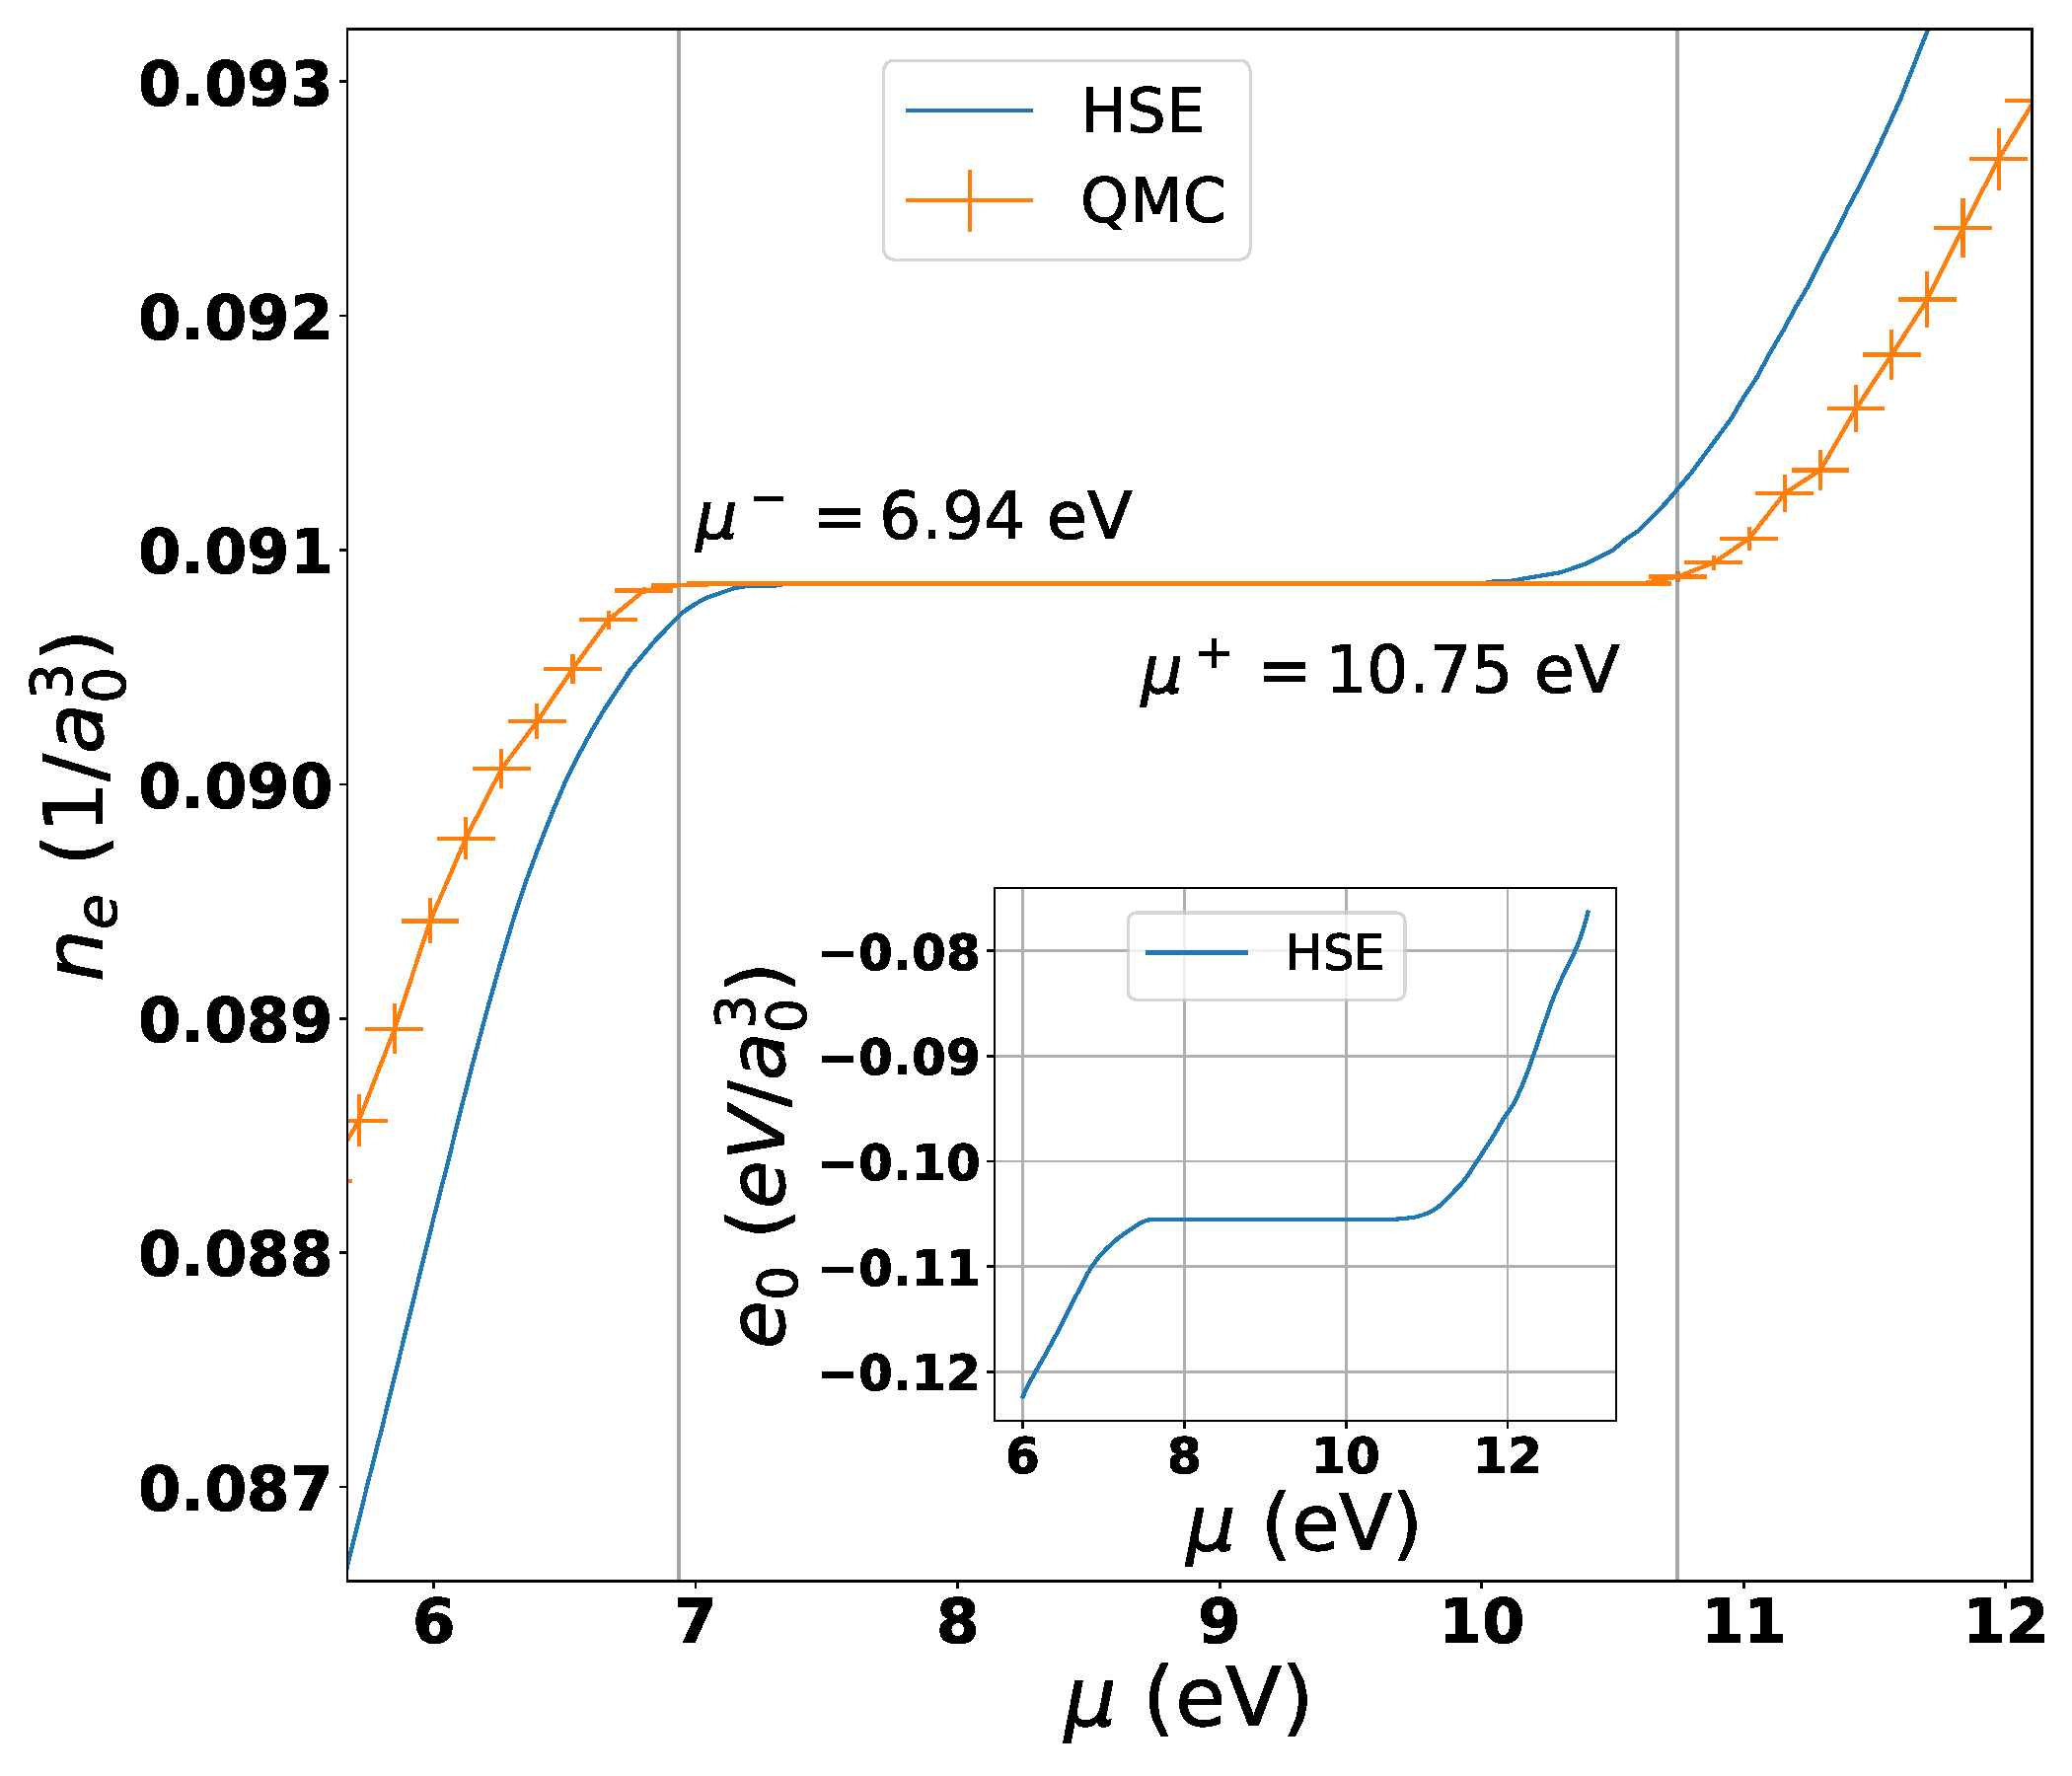
\includegraphics[width=\columnwidth]{DFT_RQMC_C2CP250dVs}
(a) 
\end{minipage}
\begin{minipage}[b]{0.49\columnwidth}
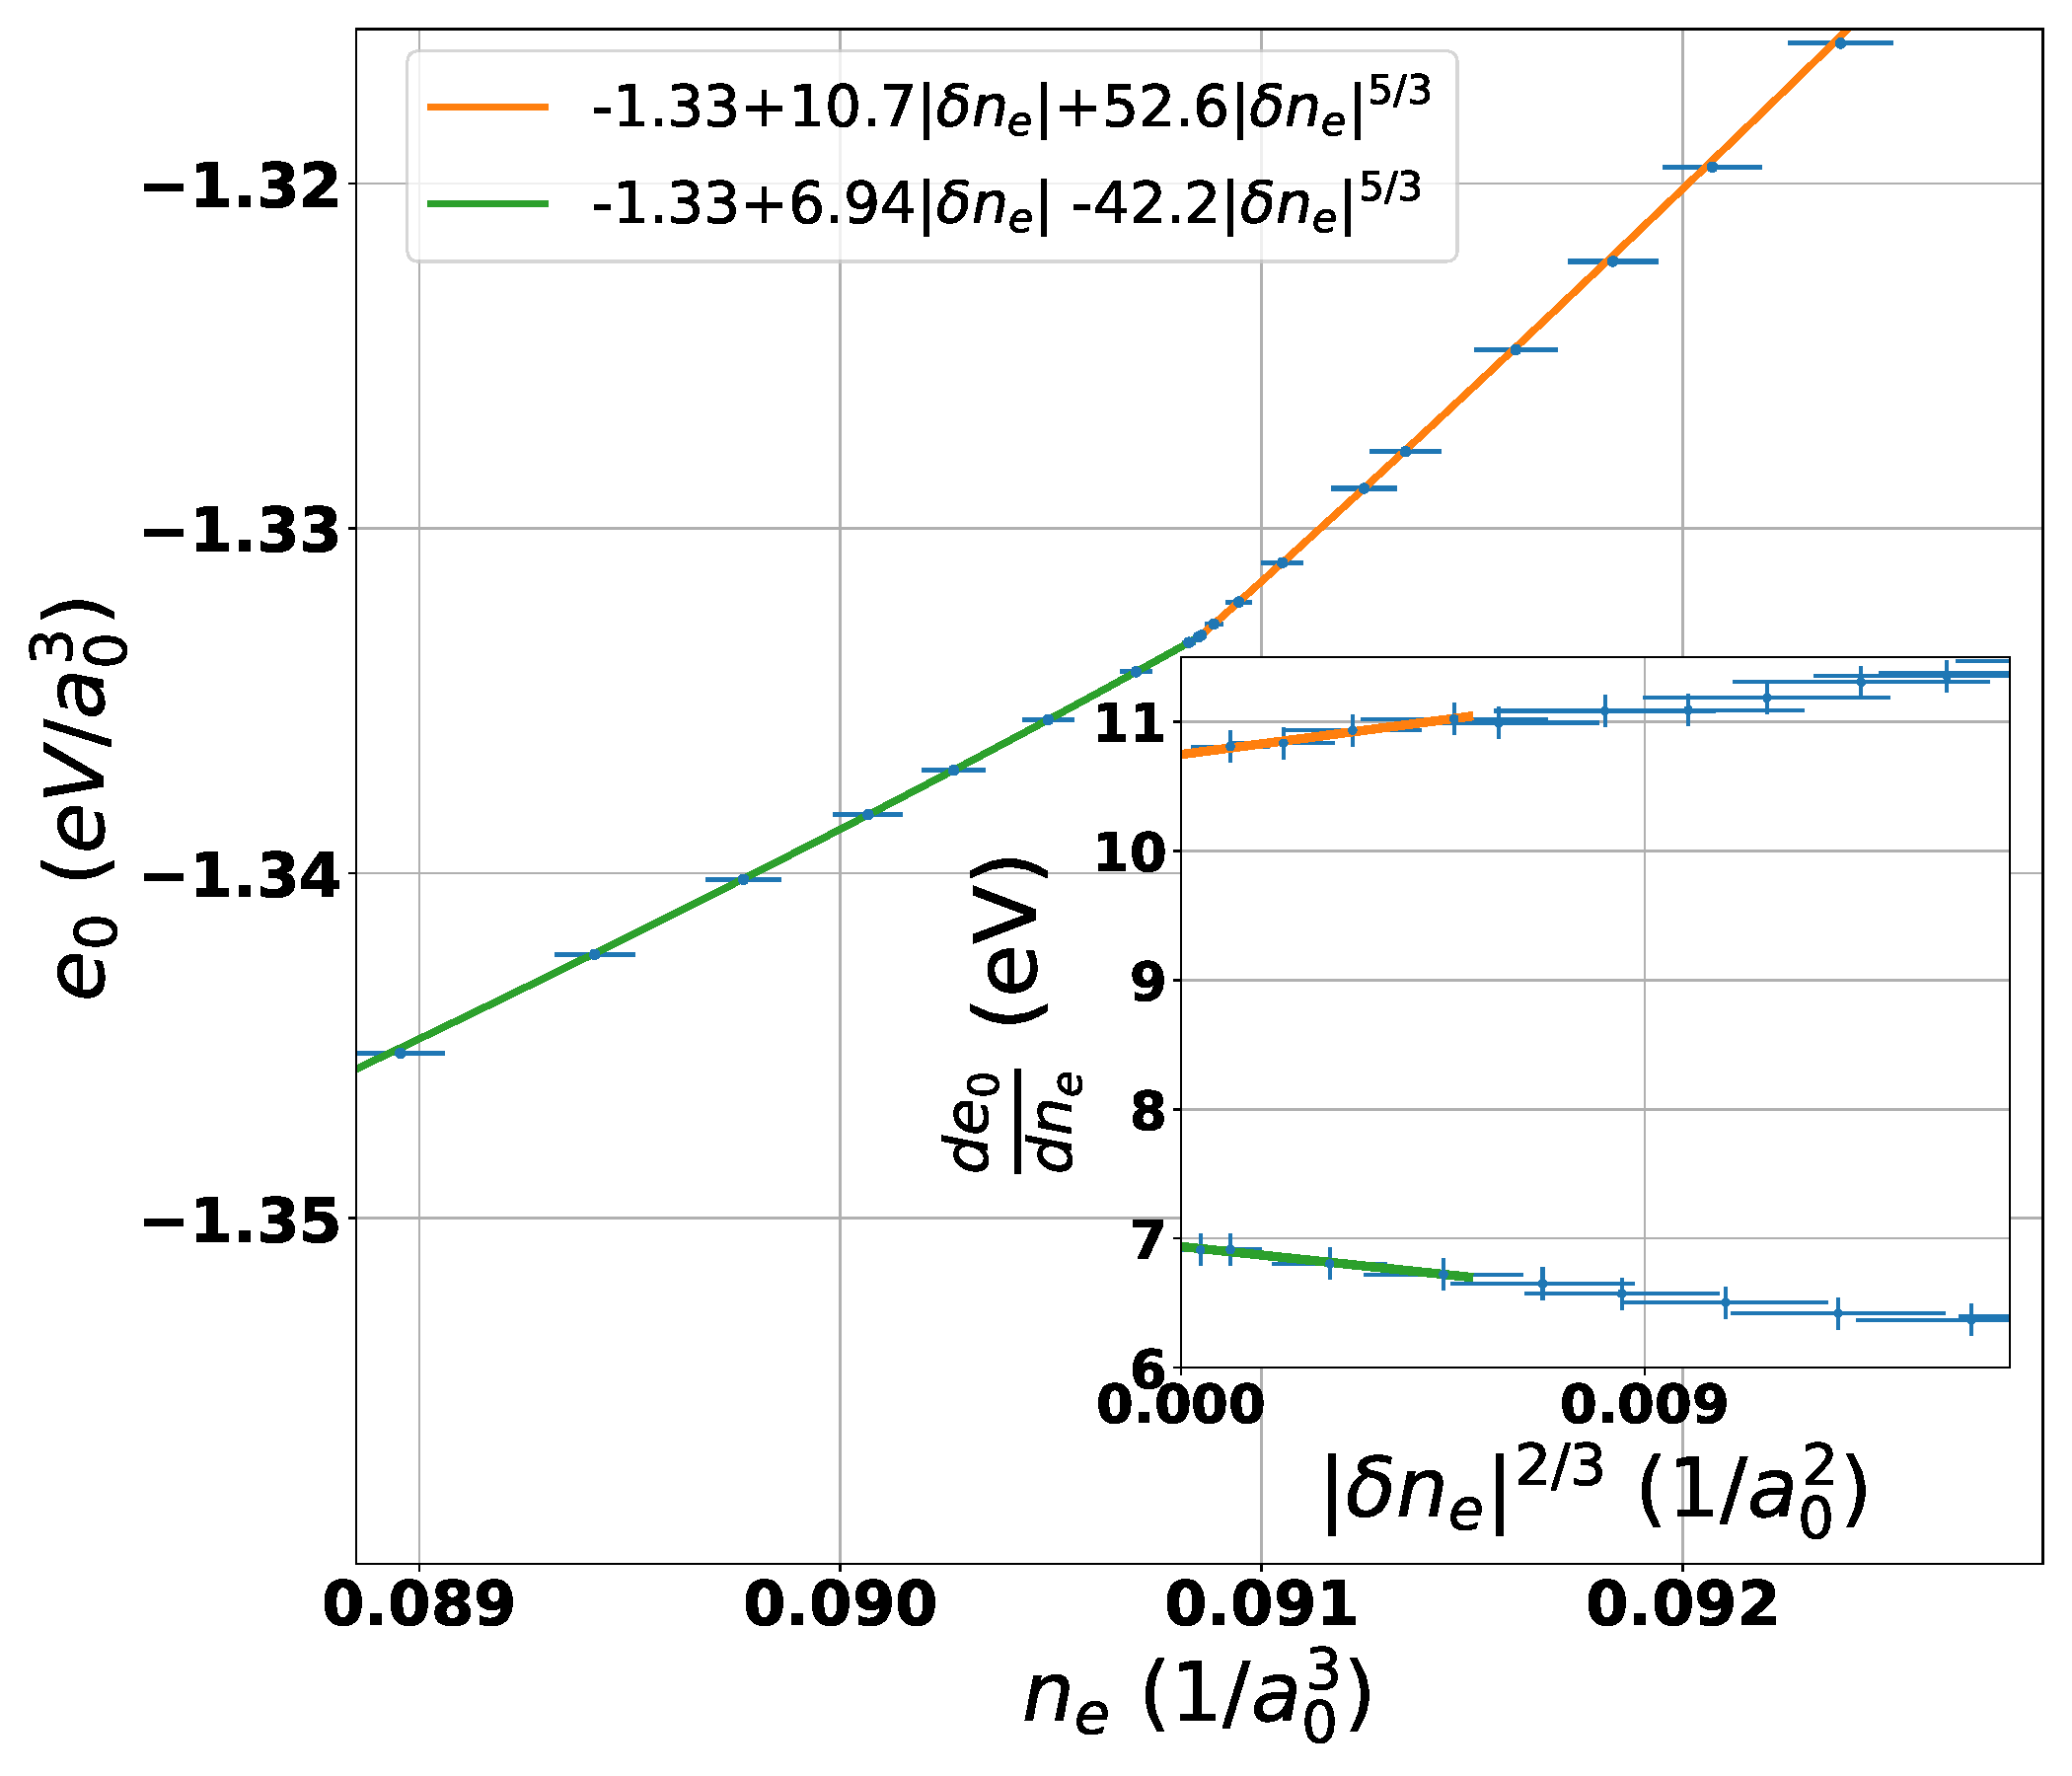
\includegraphics[width=\columnwidth]{RQMC_C2CP250dVs}
(b) 
\end{minipage}
\caption{GCTABC analyses of the C2/c-24 structure of solid hydrogen at $r_s=1.38$ (234GPa). (a) 
The electron density, $n_e$, as a function of the chemical potential $\mu$ obtained from HSE functional
in comparison to QMC; the inset illustrates the energy density, $e_0$, as a function of $\mu$ from HSE functional.
(b) Energy density, $e_0$, as a function of $n_e$ using QMC; the inset shows the derivative discontinuity where $\delta n_e$ is the change of the electronic density with respect to the insulating state.
Size corrections as discussed in the text are included.
 \label{fig:H_C2CP250}}
\end{figure*}

\section{Finite size effects\label{sec:bg-fse}}

\subsection{Potential energy}

A key quantity in understanding size effects is the long wavelength behavior of the static structure factor,
$S_{N_e}(\kvec)=\langle \rho_{-\kvec} \rho_{\kvec} \rangle/N_e$, where $\rho_\kvec=\sum_j e^{i \kvec \cdot \rvec_j}$ is the Fourier transform of the instantaneous electron density.
The structure factor for a homogeneous system obeys the bound \cite{Ceperley87,book},
\beq
S_{N_e}(k) \le \frac{\hbar k^2}{2m \omega_p}\left( 1 - \frac{1}{\epsilon_k} \right)^{1/2},
\label{davidbound}
\eeq
where $\omega_p=4 \pi \hbar^2 e^2 n_e/m$ is the plasma frequency and $\epsilon_k$ the static dielectric constant for wavevector $k$ (to simplify the notations, we will suppress the dependence on the wave vector in the following). This inequality is derived by applying the plasmon-pole approximation to the sum rules of the dynamic structure factor $S(k, \omega)$. It implies that the structure factor must vanish quadratically as
$k \rightarrow 0$ \cite{Nozieres}.
Equality will be obtained if $S(k,\omega)$ reduces to a single delta function at small $k$.
The $1/N_e$ finite-size corrections of the energy per electron is a direct consequence of
this behavior of $S_{N_e}(k)$ \cite{fse}. However, these leading order corrections are not sufficient for excitation energies, since the energy gap is of the same order as finite-size corrections to the total energy.

As we will show below, the key to understanding size effects of energy differences is encoded in the change of $S_{N_e}(k)$ as electrons are added or removed. In particular, the limiting behavior of $S_{N_e\pm 1}(k)$ as $k\rightarrow0$ will provide the dominant finite-size correction.

For concreteness, we will assume a Slater-Jastrow form for the ground-state wave function
$\Psi_0 \propto D \exp[-U]$. The determinant, $D$, is built out of Bloch orbitals, $\phi_{\qvec n}(\rvec)$ with $\qvec$ inside the first Brillouin zone, $n$ is the band index, and $U$ is a general, symmetric $n$-body correlation factor \cite{nbody}. For simplicity, we assume it is two body: $U=\sum_{i<j} u(r_i,r_j)$.  
Let us consider the action of $e^{i \kvec \cdot \rvec_j}$ on a single-particle orbital
$\phi_{\qvec n}(\rvec_j)$ in the Slater determinant of the ground state.
In the limit of small $\kvec$,  
this can be approximately written as $ \phi_{\qvec+\kvec n}(\rvec_j)$.
Expanding the determinant in terms of its cofactors $\frac{\delta D}{\delta \phi_{\qvec n}(\rvec_j)}$ and making the excitation, we have
\beq
\rho_\kvec \Psi_0
\propto \sum_j \sum_{\qvec,n} \frac{\delta D}{\delta \phi_{\qvec n}(\rvec_j)} e^{i \kvec \cdot \rvec_j}
 \phi_{\qvec n}(\rvec_j) e^{-U}.
\eeq
and the resulting determinant after summation over $j$
vanishes for small $k$ if the Bloch orbital $(\qvec+\kvec,n)$
is already occupied in the ground-state determinant.
Considering $N_e \pm 1$ electron wave functions, $\Psi_0(N_e \pm 1; \pm \qvec,  m)$, where $N_e$ corresponds to the insulating state
with fully occupied bands in the Slater determinant, and $\qvec m$ denotes the additional particle/
hole orbital, we get
\beq
\lim_{k \to 0} \rho_\kvec \Psi_0(N_e \pm 1;\qvec, m)  
\sim \pm \Psi_0(N_e \pm 1;\qvec + \kvec, m)
\label{limitk}
\eeq
for $k \ne 0$, where different signs for particle or hole excitations on the r.h.s. are chosen to match 
the most common sign convention, e.g., of Ref.~\cite{Kohn58}. The limit $k \to 0$ is discontinuous since 
$\rho_{\kvec=0} \Psi_0(N_e \pm 1;\qvec, m)\equiv (N_e \pm 1)\Psi_0(N_e \pm 1;\qvec, m)$.

Kohn \cite{Kohn57,Kohn58} has pointed out that in the insulating state, the matrix elements
\bea
\lim_{\qvec' \to \qvec} \langle \Psi_0(N_e \pm 1;\qvec, m) | \rho_{\qvec-\qvec'} |
\Psi_0(N_e \pm 1;\qvec', m) \rangle = \pm \frac1{\epsilon}
\nonumber
\label{kappastar}
\\
\eea
approach the inverse dielectric constant, $\epsilon^{-1}$, up to a sign.

Substituting Eq.~(\ref{limitk}) into Eq.~(\ref{kappastar}), suggests 
the following finite-size behavior of the static structure factor of insulators
\beq
\lim_{k \to 0} S_k^{\pm}
= \alpha_{\pm} +{\cal O}(k^2),
\label{sqeps}
\\
S_k^{\pm} \equiv (N_e \pm 1) S_{N_e \pm 1}(k) - N_eS_{N_e}(k),
\eeq
where $\alpha_\pm$ is proportional to $\epsilon^{-1}$. However, $\alpha_\pm$ in general differs from $\epsilon^{-1}$ unless Eq.~(\ref{limitk}) is an exact equality.

Figure \ref{fig:c-si-skpm} shows the behavior of $S_k^{\pm}$  
for carbon and silicon crystals. Note that these functions extrapolate to a nonzero value as $k \rightarrow 0$.

The long wavelength behavior of the structure factor, Eq.~(\ref{sqeps}), then gives rise to size
corrections to excitation energies through the potential energy term
\beq
\left[ \int \frac{d^3 k}{(2 \pi)^3}  -   \frac{1}{V} \!\sum_{\kvec \ne 0} \right]
 \frac{v_k}{2} S_k^{\pm}
\simeq  \alpha_{\pm} \frac{|v_M|}{2}, 
\label{eq:vk-skeps}
\eeq
where we have defined the Madelung constant as
\beq
v_M= 
\left[ \frac{1}{V} \sum_{\kvec \ne 0} - \int \frac{d^3 k}{(2 \pi)^3}\right] v_k
\sim L^{-1} \sim N_e^{-1/3}.
\label{vMdef}
\eeq
For the Coulomb potential, $v_M$ is proportional to $L^{-1}$, the inverse linear extension of the simulation cell. The negative proportionality constant  depends on the boundary conditions, e.g., cell geometry, and can be calculated by the Ewald image technique \cite{Ewald}.

\subsection{Kinetic energy}

Following Ref.~\cite{finitesize}, we now discuss the kinetic energy
contribution $\hbar^2 [\nabla U]^2/2m$ which arises from electron correlation.
For a two-body Jastrow, $U=\sum_\kvec u_k \rho_\kvec  \rho_{-\kvec}/2 V$, and we are only
interested in the long-wavelength limit, $k \to 0$, of the electron-electron 
correlation, with wave vectors smaller than the reciprocal lattice vectors
of the crystal, $\Gvec$.
Isolating the singular contributions involving $\rho_{k=0} \equiv N_e$ 
in the spirit of the rotating (random) phase 
approximation (RPA) we have
\bea
\left\langle \left[\nabla U \right]^2 \right\rangle
&=& - \frac{1}{V^2} \sum_{\kvec \ne 0, \kvec' \ne 0}
(\kvec \cdot \kvec') u_k u_{k'} \langle \rho_{\kvec+\kvec'} \rho_{-\kvec} \rho_{-\kvec'} \rangle
\nonumber \\
&\simeq&
\frac{1}{V^2} \sum_{\kvec \ne 0}
 N_e
k^2 u_k^2 \langle \rho_\kvec \rho_{-\kvec} \rangle.
\eea
Therefore,
for systems with explicit long-range correlations $u_k \sim k^{-2}$, the kinetic energy will also
contribute to the leading order size corrections with 
\begin{eqnarray}\label{eq:uk-sqeps}
\left[ \int \frac{d^3 k}{(2 \pi)^3}  -  \frac{1}{V} \sum_{\kvec \ne 0} \right]
 \frac{n_e \hbar^2 k^2u_k^2}{2m}  S_k^\pm
\simeq  \alpha_\pm c \frac{|v_M|}{2},
\end{eqnarray}
where $c= \lim_{ k \to 0} n_e \hbar^2 k^2u_k^2/(mv_k)$ is approximately given by the ratio of the $1/N_e$ finite-size
corrections of the kinetic to potential energy of the ground state energy per particle due to
two-body correlations \cite{finitesize}.

\subsection{Total gap corrections from Coulomb singularity}

Up to now, we have shown how the long-range behavior of the structure factor and Jastrow factor can give rise
to a $1/L$ correction to the excitation gap with a proportionality factor determined
by the structure factor changes.
In the following, we will further demonstrate that, given that the trial wave functions coincide with
the exact ground-state wave function for $N_e$ and $N_e \pm 1$ electrons,
this proportionality factor is indeed given by the dielectric constant 
\beq
\Delta_\infty - \Delta_V = \frac{|v_M|}{\epsilon}+ {\cal O}\left( \frac1V \right),
\label{gapepsilon}
\eeq
as phenomenologically
assumed in previous work \cite{Engel,Hunt}.

We prove this by an independent argument based on commutation relations.
Let us denote the exact insulating ground state of the $N_e$ electron system as $|\Psi_0^{N_e} \rangle$, its energy as $E_0^{N_e}$, and the exact excited state of the $N_e\pm 1$ electron system as $|\Psi_\kvec^{N_e\pm 1} \rangle$ with energy $E_\kvec^{N_e\pm 1}$; $\kvec$ indicates that the additional/subtracted electron adds/subtracts the crystal momentum $\kvec$.
We have
\beq
E_\kvec^{N_e+ 1} - E_0^{N_e}
= \frac{ \langle \Psi_\kvec^{N_e+1} | \left[ H,a_\kvec^\dagger \right] |\Psi_0^{N_e} \rangle}
{\langle \Psi_\kvec^{N_e+1} | a_\kvec^\dagger |\Psi_0^{N_e} \rangle}
\eeq
for particle and
\beq
E_\kvec^{N_e- 1} - E_0^{N_e}
= \frac{ \langle \Psi_\kvec^{N_e-1} | \left[ H,a_\kvec \right] |\Psi_0^{N_e} \rangle}
{\langle \Psi_\kvec^{N_e-1} | a_\kvec |\Psi_0^{N_e} \rangle}
\eeq
for hole excitations.
In second quantization, the Hamiltonian, 
$H=T+V_{ee}$, is given by
\bea
T &=& \sum_\kvec \left[ \frac{\hbar k^2}{2m} a_\kvec^\dagger a_\kvec 
+ \sum_\Gvec u(\Gvec) a_{\kvec+\Gvec}^\dagger a_\kvec \right],
\\
V_{ee}&=&\frac{1}{2 V} \sum_{\qvec \ne 0}
v_q \left[\rho_\qvec \rho_{-\qvec} - N_e\right],
\eea
where $a_\kvec$ is the annihilation operator for plane-wave states of wave vector $\kvec$,
$u(\Gvec)$ the periodic crystal potential, and $v_q$ is the Coulomb potential
between electrons, $\rho_\qvec= \sum_\kvec a_{\kvec+\qvec}^\dagger a_\kvec$,
and $N_e=\sum_k a_\kvec^\dagger a_\kvec$.

The commutator involving the single-particle energy term is
\beq
\left[ T, a_\kvec^\dagger \right]
= \frac{\hbar^2 k^2}{2m} a_\kvec^\dagger + \sum_\Gvec u(\Gvec) a_{\Gvec+\kvec}^\dagger.
\eeq
There are corresponding terms for hole excitations, but none of these terms 
involve singular contributions responsible for anomalous size effects, so
these terms do not contribute at leading order.
However,
\beq
\left[ V_{ee}, a_\kvec^\dagger \right]
= \frac{1}{V} \sum_{\qvec \ne 0} v_q 
\left[\rho_\qvec a_{\kvec-\qvec}^\dagger -1 \right]
\label{Veecom}
\eeq
and
\beq
\left[ V_{ee}, a_\kvec \right]
= -\frac{1}{V} \sum_{\qvec \ne 0} v_q 
\rho_\qvec a_{\kvec+\qvec}
\eeq
involve terms approaching the Coulomb singularity, $v_q \sim q^{-2} \to \infty$ for $q \to 0$.

From these terms, we get the leading order size corrections by noting that
\bea
\lim_{\kvec, \qvec \to 0}
\frac{\langle \Psi_{\kvec}^{N_e+1} | \rho_\qvec a_{\kvec-\qvec}^\dagger | \Psi_0^{N_e} \rangle}
{\langle \Psi_{\kvec}^{N_e+1} |
 a_{\kvec}^\dagger | \Psi_0^{N_e} \rangle}
=
\frac{1}{2}\left[\frac{1}{ \epsilon} +1 \right]
\eea
and
\bea
\lim_{\kvec, \qvec \to 0}
\frac{\langle \Psi_{\kvec}^{N_e-1} | \rho_\qvec a_{\kvec+\qvec} | \Psi_0^{N_e} \rangle}
{\langle \Psi_{\kvec}^{N_e-1} |
 a_{\kvec} | \Psi_0^{N_e} \rangle}
=
-\frac12 \left[1+ \frac{1}{\epsilon}\right].
\eea
Both relations can be obtained \cite{footnote} by extending Kohn's diagrammatic approach 
\cite{Kohn58} (see Supplemental Material~\cite{supp}).
Integrating around the $v_q$ singularity for small $q$ in Eq.~(\ref{Veecom}),
we obtain the leading order finite size corrections. As before, this involves the Madelung constant,
Eq~(\ref{vMdef}).
In the particle channel, we get
$\frac{|v_M|}{2} \left(\frac{1}{\epsilon} - 1 \right)$ and
in the hole channel, $\frac{|v_M|}{2} \left(\frac{1}{\epsilon} + 1 \right)$.
The corrections independent of $\epsilon$ correspond to the change in the background charge which
cancel for the fundamental gap and we obtain Eq.~(\ref{gapepsilon}).

Previous, heuristic approaches \cite{Hunt} have suggested that one can use
experimental or DFT values of the dielectric constant for finite-size extrapolation.
Our approach further suggests that this value can be determined from
the QMC structure factor extrapolated to zero wave vector
\beq
\frac{2}{\epsilon} \equiv (1+ c) \lim_{N_e \to \infty} \lim_{k \to 0}
\left[S_k^+ + S_k^- \right],
\eeq
with the singular behavior of the Jastrow factor determining $c$.
We emphasize that the order of the limits involved above is crucial.

An independent estimate is
based on the inequality of Eq.~(\ref{davidbound}). We can
bound and estimate the value of dielectric constant 
using the structure factor of the insulating ground state. By extrapolating $1-\Gamma_k^2$ vs. $k$ to $k=0$ we obtain an upper bound to the inverse dielectric constant, where $\Gamma_k\equiv 2m\omega_p S_{N_e}(k)/\hbar k^2$.
This involves only the extensive part
of the density-density correlations, thus, it is less sensitive to noise
and has much smaller statistical uncertainty.
In Fig.~\ref{fig:c-si-gk}, we show that for C and Si, this inequality gives accurate values of the dielectric
constant.
% si44a/gkfit.py

\subsection{Twist correction of two-particle correlations}

The above size effects explain the leading order $1/L$ correction to the single-particle gap.
However, as we will see in our results, 
the asymptotic region, where this law
can be reliably applied, may still be difficult to reach for
currently used system sizes and next-to-leading order effects are important.
Here, we show that an important part can be corrected for, by further restoring the full symmetry
properties in the contribution of the direct Coulomb interaction.

For inhomogeneous systems, it is convenient to separate the mean density from its
fluctuating components in the
static structure factor \cite{finitesize}, i.e.,
\bea
S_{N_e}(\kvec) &= &\frac{1}{N_e} \langle \rho_\kvec \rangle \langle \rho_{-\kvec} \rangle + \delta S_{N_e}(\kvec),
\\
\delta S_{N_e}(k) &=& \frac{1}{N_e} \left\langle \left( \rho_\kvec - \langle \rho_\kvec \rangle \right),
\left( \rho_{-\kvec} - \langle \rho_{-\kvec} \rangle \right) \right\rangle.
\eea
For crystals with periodic density distributions, the Fourier components
of the mean density, $\langle \rho_\kvec \rangle$, only contribute for reciprocal lattice vectors, $\kvec \in \Gvec$. The long wavelength behavior of the structure factor is entirely
due to the fluctuating part $\delta S_{N_e}(k)$, which therefore contains the leading order
size effects \cite{finitesize}. However, the mean 
single particle density,
$\langle \rho(\rvec) \rangle=V^{-1} \sum_\kvec \langle \rho_\kvec \rangle e^{i \kvec \cdot \rvec}$, of the finite system may significantly differ from  the infinite one, particularly
in cases where the supercell is not compatible with the full symmetry group of the crystal.

Averaging over twisted boundary conditions is designed to restore the symmetry of the crystal,
thus accelerate the convergence of single-particle
densities to the thermodynamic limit. In the following, we denote the twist averaged  expectation value by
\beq
\overline{ {\cal{O} }} \equiv \frac{1}{M_\theta} \sum_{\theta} 
\langle {\cal{O}} \rangle_{N_e, \theta},
\eeq
where we have explicitly indicated the $N_e$ and $\theta$ dependence on the expectation value
on the r.h.s. For any single-particle theory, $\overline{\rho( \rvec )}$ approaches its thermodynamic
limit for calculations at fixed $N_e$  by
averaging over a dense grid of twist angles ($M_\theta \to \infty$). % due to Bloch's theorem.
Within many-body calculations, twist-averaging \cite{Lin01} takes over a large part of this
property to any observable {\em linear} in the density. Here, we extend this approach to
also correct the quadratic expression entering the two-body contributions
of the total energy.

For the potential energy, this correction to the twist-converged QMC calculation is
\bea
\delta V_{N_e}^s &= &
 \frac1{2V} \sum_\kvec v_k \delta C(\kvec), \nonumber \\
&&\delta C(\kvec) =
\overline{\rho_\kvec } \, \overline{\rho_{-\kvec}}
- \overline{\rho_\kvec \rho_{-\kvec}} .
\label{deltaV}
\eea
For the ground-state energies, this correction provides only a small improvement over our previous correction~\cite{fse,finitesize}.

For the gap, many terms entering Eqs.~(\ref{deltaV}) cancel and the expression can be simplified. Let us consider the case of adding/removing one electron at twist $\phi$ to
the insulating ground state, denoting $\Pi_\kvec^{\pm}$ the difference of the respective densities:
\begin{equation}
\Pi_\kvec^{\pm} \equiv
\langle \rho_\kvec  \rangle_{N_e \pm 1,\phi} - \langle \rho_\kvec  \rangle_{N_e,\phi}
\end{equation}
In the thermodynamic limit, the density of the ground-state system with $N_e$ electrons
coincides with the twist-averaged ground-state density $\overline{\rho_\kvec}$, whereas
we obtain $\overline{\rho_\kvec}+\Pi_\kvec^{\pm}$
for the density of the $N_e \pm 1$ electron system.
Inserting into Eqs.~(\ref{deltaV}), we obtain the correction for the difference between the two states,
\begin{equation}
\delta V_{N_e \pm 1,\phi}^s - \delta V_{N_e}^s
= \frac{1}{V} \sum_{\kvec\in \Gvec} v_k \text{Re}
\left[ \left( \overline{\rho}_\kvec
- \langle \rho_\kvec \rangle_{N_e,\phi} \right) \Pi_{-\kvec}^{\pm}
\right],
\label{twistadd}
\end{equation}
where only wave vectors of the reciprocal crystal lattice contribute
to the sum.
The corresponding finite size correction for the gap,
denoted by $\delta \Delta_s$ in the following,
is order $1/N_e$ or smaller, mainly determined by the changes
of the ground-state densities at the first Bragg-peaks due to twist averaging.

Equation~(\ref{twistadd}) can be understood quite intuitively: It corrects the
direct Coulomb interaction between the electron/hole in the
excited state ($\Pi^\pm$) with the unexcited electrons. The density
of those electrons is expected to change
by $\overline{\rho}_\kvec - \langle \rho_\kvec \rangle_{N_e,\phi}$
in the thermodynamic limit.

Converged ground-state densities are naturally calculated within
GCTABC.  It is straightforward to apply the correction Eq.~(\ref{twistadd})
to all excitation energies.
Alternatively, the corresponding
 DFT densities may be used. This removes the stochastic error at the cost of
introducing a small bias in the next-to-leading order size correction.

\begin{figure*}
\begin{minipage}[b]{0.49\columnwidth}
\centering
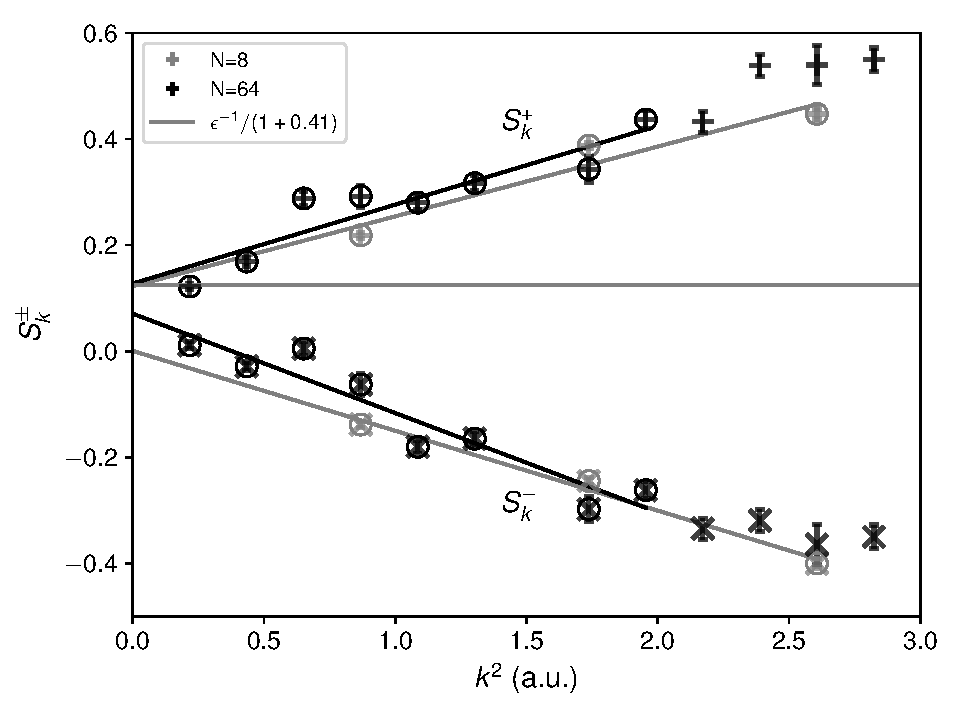
\includegraphics[width=\columnwidth]{si30c_skpm-ceps-c-k2-fit}
(a) carbon
\end{minipage}
\begin{minipage}[b]{0.49\columnwidth}
\centering
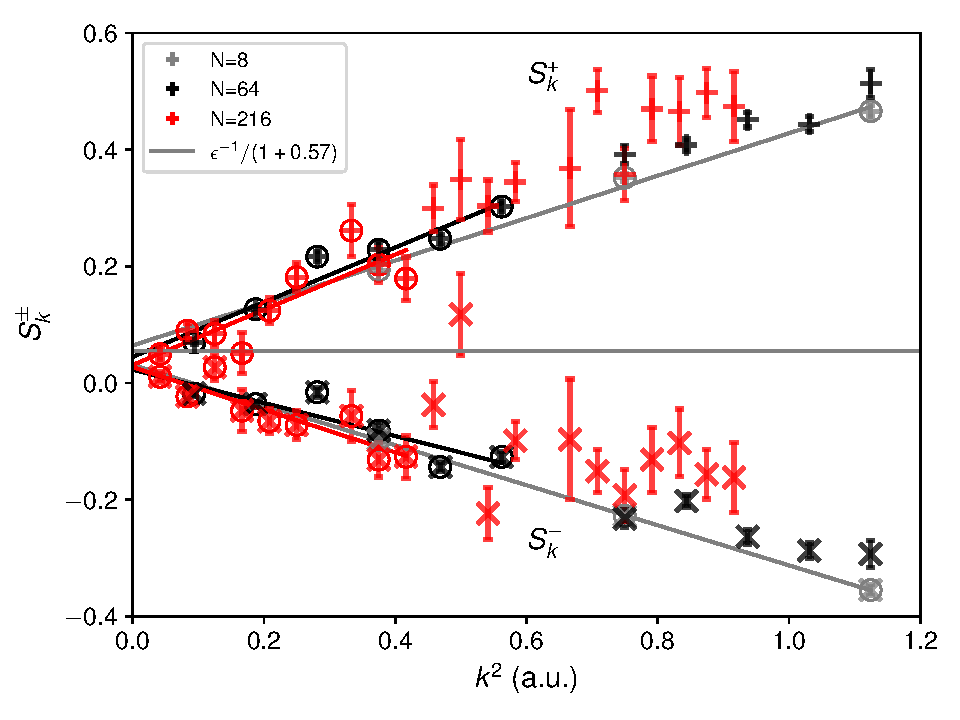
\includegraphics[width=\columnwidth]{si30c_skpm-ceps-si-k2-fit}
(b) silicon
\end{minipage}
\caption{Change in the static structure factor as an electron (upper curves) or a hole (lower curves) is added to the insulating system with $N$ atoms. %Circled points are used to obtain a linear (in $k^2$) fit of matching color.
The lines are fits to the data points.
The horizontal lines show the expected $k\rightarrow0$ limit based on the experimental dielectric constants. We have used $c=0.41$ for C and $c=0.57$ for Si.
\label{fig:c-si-skpm}}
\end{figure*}

\begin{figure*}
\begin{minipage}[b]{0.49\columnwidth}
\centering
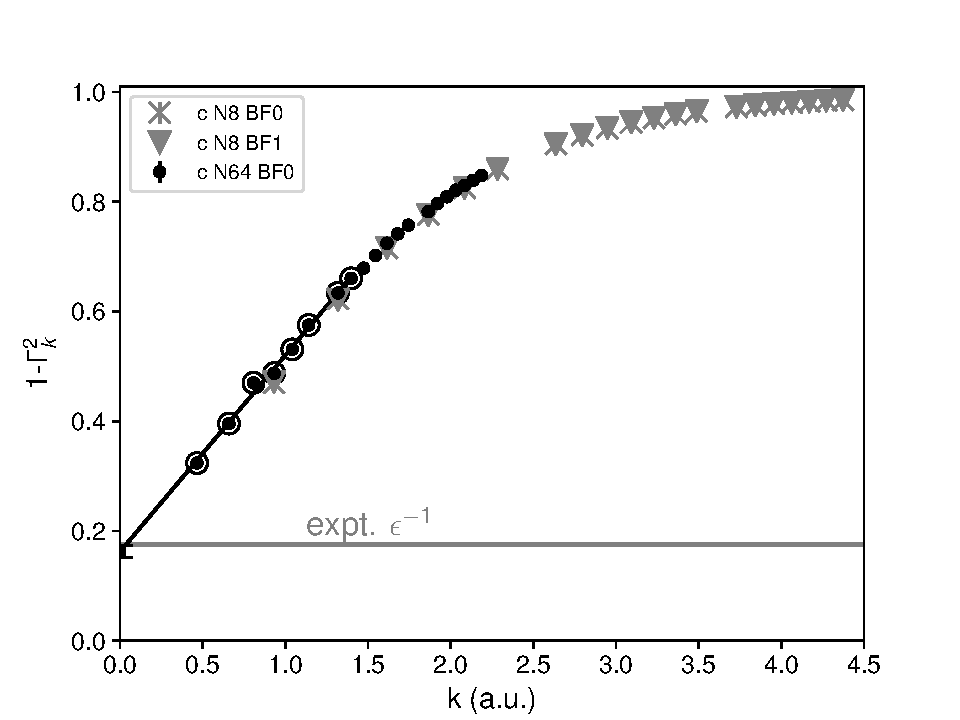
\includegraphics[width=\columnwidth]{si45_uksk-c-gk2}
(a) carbon
\end{minipage}
\begin{minipage}[b]{0.49\columnwidth}
\centering
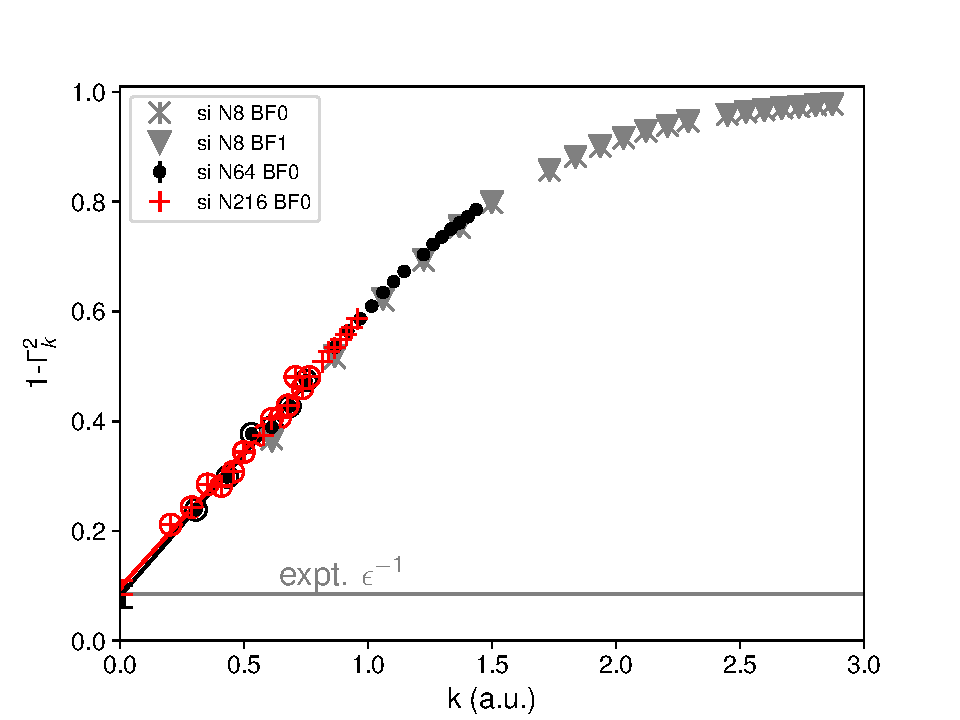
\includegraphics[width=\columnwidth]{si45_uksk-si-gk2}
(b) silicon
\end{minipage}
\caption{Upper bound to the inverse dielectric constant  Eq.~(\ref{davidbound}), where $\Gamma_k\equiv\frac{2m\omega_pS_{N_e}(k)}{\hbar k^2}$. Lines are fits to the low-$k$ data. %The 8-atom cells have few points in the linear region of $1-\Gamma_k^2$, so we did not use them to estimate $\epsilon^{-1}$. 
The horizontal lines mark experimental inverse dielectric constants.
\label{fig:c-si-gk}}
\end{figure*}

\section{Computational methods\label{sec:bg-methods}}

We have performed electronic QMC calculations on three insulating solids:
molecular hydrogen at high pressure,
and carbon and silicon in the diamond structure at zero pressure. Since we are interested in the
spin-neutral charge gap, we used an equal number of spin-up and spin-down electrons. We used a Slater-Jastrow  trial wave function with backflow (BF) corrections \cite{Holzmann2003,Trial}. The Jastrow and BF functions were fully optimized within variational Monte Carlo, including the long-range (reciprocal lattice) contributions.
The orbitals in the Slater determinant were taken from DFT calculations using Quantum Espresso~\cite{QE2009, QE2017}. The carbon and silicon orbitals were generated using the LDA functional, whereas the hydrogen orbitals were generated using the PBE functional, which has been shown to provide a good trial QMC wave function \cite{Morales2012,Pierleoni2016}.

Molecular hydrogen was placed in the C2/c-24 structure \cite{Pickard2007} at two different densities ($r_s=1.38$ and $r_s=1.34$), roughly corresponding to pressures of 234 GPa and 285 GPa, respectively.
Energies and structure factors were obtained from reptation Quantum Monte Carlo calculations using the BOPIMC code \cite{BOPIMC}. For carbon and silicon, DMC calculations have been performed with the QMCPACK code \cite{QMCPACK}
at the experimentally measured zero pressure valence densities, $r_s=1.318$ and $r_s=2.005$, respectively.
The crystal structures were optimized by DFT using the vdW-DF1 functional.
For hydrogen, the QMC calculations have been done with the bare Coulomb interaction. The PAW pseudo-potential has been used for the DFT results shown in Fig.~\ref{fig:H_C2CP250}. For carbon and silicon, pseudopotentials were used to remove the core electrons: carbon ions modeled by the Burkatzki-Filippi-Dolg pseudopotential~\cite{Burkatzki2007}, and silicon ions by the Trail-Needs pseudopotential~\cite{Trail2005}. These are considered good pseudo-potentials for correlated calculations, but their use within DFT calculations produces slightly different results from the literature even with the same functional.
For hydrogen, we used a supercell with  $2 \times 2 \times 1$ primitive cells so the supercell is nearly cubic and contained 96 protons. For carbon, we used two system sizes: the cubic cell containing 8 atoms and a $2\times 2\times 2$ supercell containing 64 atoms. For silicon, in addition to these systems, we used a $3\times 3\times 3$ supercell containing 216 atoms.
For hydrogen, the twist convergence has been achieved using a $8 \times 8 \times 8$ twist grid. For C and Si, the twist grid density decreases with increasing system size. The Supplemental Material~\cite{supp} contains the QMC calculated energies and variances of the insulating ground states
of the various systems obtained after twist averaging and two-body finite size corrections.

\section{Results\label{sec:bg-results}}

For any effective single-particle theory, such as Kohn-Sham DFT,
the densities and energies, $n_e(\mu)$ and $e_0(\mu)$,
are obtained by occupying all single-particle states below the chemical potential $\mu$.
By construction, the gap, as determined from the incompressible region of $n_e(\mu)$ or from the discontinuity in the derivative of $de_0/dn_e$ (see Fig.~\ref{fig:H_C2CP250}), then coincides with the one obtained from the band structure.

The LDA band gaps of carbon and silicon in the diamond structure are indirect and lie along the $\Gamma X$ direction where $\Gamma$ is the origin of the Brillouin zone and
$X$ the Brillouin zone boundary in the $(100)$ direction. By looking directly at the highest-occupied molecular orbital (HOMO) and lowest unoccupied molecular orbital (LUMO) states with LDA, it is found that
the carbon gap is 3.89 eV %for our pseudopotential LDA calculation %involves the hole state
%at ($\Gamma$, 13.30 eV) and the particle excitation at (0.75$\Gamma X$, 17.19 eV), whereas
and the silicon gap is  0.34 eV.
% at ($\Gamma$, 6.36 eV) and  (0.85$\Gamma X$, 6.70 eV), respectively.
The bands immediately above and below the gap can be fit
to a quadratic form which implies $e_0(\mu) = \mu^{\pm} n_e(\mu) + b^\pm n_e(\mu)^{5/3}$. Therefore, the derivative $de_0/dn_e = \mu^{\pm} + \frac{5b^{\pm}}{3} n_e^{2/3}$ has a discontinuity at $n_e=0$ and behaves as $ n_e^{2/3}$ above and below the gap. 
Applying our GCTABC procedure to a single-particle theory,
all states with energies below the chemical potential are occupied. Varying the chemical potential
thus scans the underlying density of states. The band gap is then determined by locating the band
edges, $\mu^\pm$, disregarding the location in the Brillouin zone \cite{BrillouinFootnote}.
Figure~\ref{fig:band_edges} illustrates the density of states
obtained from GCTABC giving an LDA gap of 3.95 eV for the carbon gap
%with band edges at 13.27 eV and 17.22 eV,
and 0.38 eV for the silicon gap. % from 6.34 eV to 6.72 eV.
The small differences ($\sim 0.05$ eV) from the values obtained before are due to the finite
resolution of the twist grid, and can be controlled by using denser grids.

As can be seen in the same figure, the effective band edge densities of states from GCTABC-DMC
have a similar functional form, but with a larger gap than the DFT ones.
The QMC computed gaps
for the different sizes of the supercell are summarized in table \ref{tab:dmc-gcta-gap}.
The results from different supercells clearly show the important bias 
on gap introduced by the finite size of the supercell. In Fig.~\ref{fig:gap-extrap}, we show the bare gap, $\Delta_N$, the Madelung-corrected one, $\Delta_N+|v_M|/\epsilon$, and our best correction, $\Delta_\infty=\Delta_N+|v_M|/\epsilon+\delta \Delta_s$, for both systems against the linear size of the supercell, where $N$ is the number of atoms in the supercell and $\epsilon$ is the experimental value of the dielectric constant.
We see that the next-to-leading-order corrections are 
comparable to the leading-order one, in particular for the 8-atom supercell of Si,
whereas they rapidly decay for the larger sizes. 

\begin{figure}
\begin{minipage}{0.49\columnwidth}
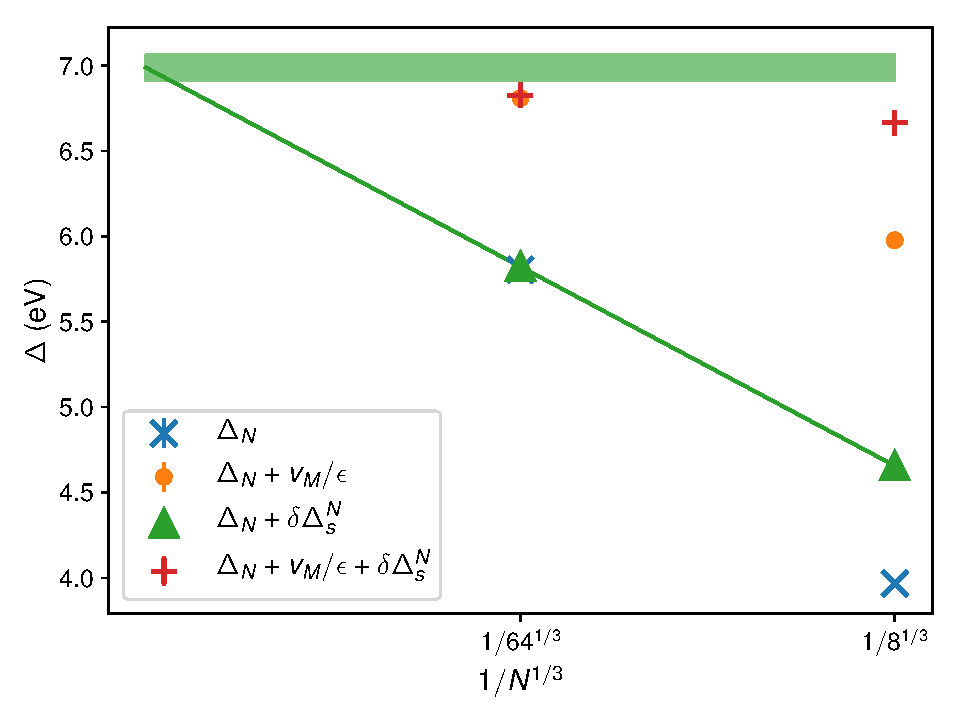
\includegraphics[width=\columnwidth]{si35f_nofold-c-nodvs-gap-extrap}
(a) carbon
\end{minipage}
\begin{minipage}{0.49\columnwidth}
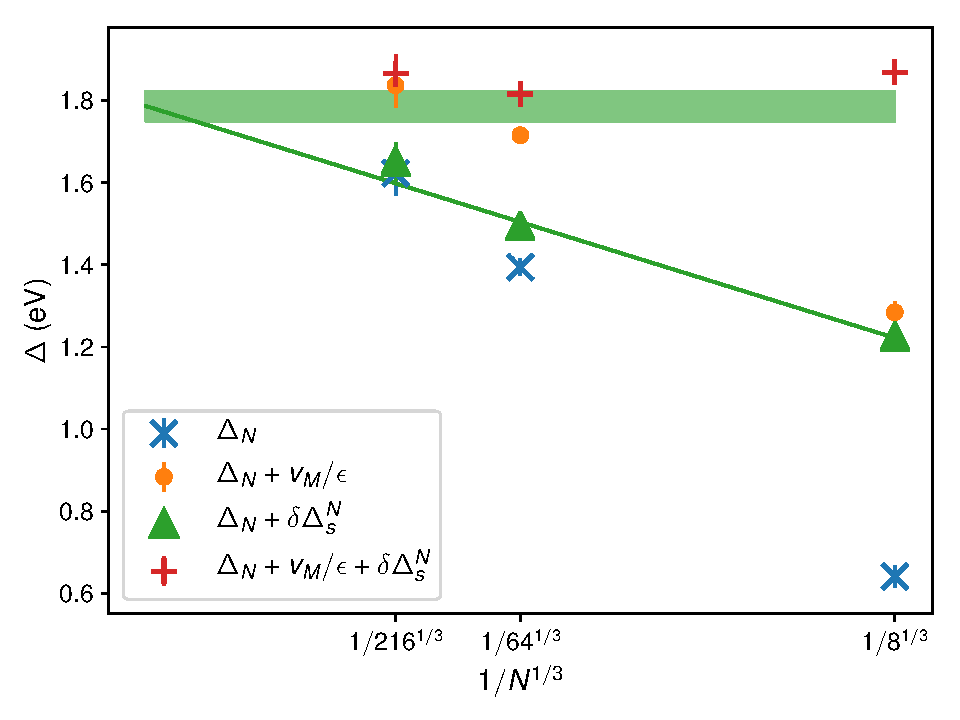
\includegraphics[width=\columnwidth]{si35f_nofold-si-nodvs-gap-extrap}
(b) silicon
\end{minipage}
\caption{Fundamental gap before and after finite-size corrections. $\Delta_N$ is the DMC gap from a simulation with $N$ atoms in the supercell without any finite-size correction, $v_M/\epsilon$ is the leading-order Madelung correction using the experimental value of $\epsilon^{-1}$,
$\delta\Delta^N_s$ is the next-to-leading-order density correction, which is related to the static part of the structure factor. The line is a fit to $\Delta_N + \delta\Delta^N_s$. \label{fig:gap-extrap}}
\end{figure}

The finite-size corrected values, $\Delta_\infty$, of all different sizes C and Si supercells agree with
each other within the statistical uncertainty, yielding the DMC-SJ values $\Delta_\infty=6.8(1)$
and  $\Delta_\infty=1.8(1)$ for the C and Si gap, respectively. 
We further note, that these values also agree with a numerical
$N^{-1/3}$ extrapolation of the gap values corrected by $\delta \Delta_s$. For any numerical
$N^{-1/3}$ extrapolation, it is very important to reduce any bias due to higher order corrections
as much as possible, since the outcome of a fit is sensitive to the smallest system sizes
since they have the smallest statistical uncertainty. For Si,
a $N^{-1/3}$ extrapolation
of the bare $\Delta_N$ values yields an overestimation of $0.3$ eV compared to $\Delta_\infty$.

Since our finite-size corrected gaps show size convergence for the smallest system size,
it is now feasible to address the systematic error due to the fixed node approximation.
To reduce this bias,
we have added BF correlations in the Slater orbitals. Our BF correlations lower
the SJ gap by $0.1$ eV for both, C and Si.
Previous BF calculations \cite{Hunt} on Si have reported a $0.2$ eV lowering compared to SJ.
The difference might be due to a different functional form or optimization procedure.
A systematic study on the bias of the fixed-node approximation such as done with more general BF correlations \cite{BFN,orbitalbf} or
multi-determinant trial wave functions \cite{Zhao19}, possible for small supercells,
could be done in the future.

So far, in our analysis of C and Si, we have imposed the experimentally known dielectric constant
in the leading order Madelung correction. As described in Sec.~\ref{sec:bg-fse},
there is no need for any external knowledge to perform the size extrapolation as the value
of the Madelung correction can be obtained from the behavior of the static structure factor,
calculable within the same QMC run, see  Figs.~\ref{fig:c-si-skpm} and \ref{fig:c-si-gk}. However, since
 the extrapolation involved introduces an additional uncertainty, we have preferred to use
the experimental values to benchmark our theory and better distinguish leading
from next-to-leading order size effects. 

Using the dielectric bound Eq.~(\ref{davidbound}) on the ground-state structure factor to determine $\epsilon$, we get $\epsilon_0=6.2\pm0.4$ for C and $\epsilon_0=10.3\pm1.3$ for Si, which are compatible with the experimental values of $5.7$ and $11.7$. The corresponding leading-order finite-size corrections on the gap of the 64-atom system are then $0.92\pm0.06$ eV for C and $0.36\pm0.14$ eV for Si using the \emph{ab initio} $\epsilon^{-1}$, as opposed to $1.00$ eV for C and $0.32$ eV for Si based on the experimental values of $\epsilon^{-1}$.

As shown in Fig.~\ref{fig:c-si-skpm}, the asymptotic values of the finite-sized structure factors,
$S_k^\pm$, are affected by a much larger uncertainty, introducing larger systematic bias when
used for \emph{ab-initio} size corrections. Still, already the extrapolation to a non-zero
value fixes the leading order size corrections to decay as $1/L$. This information alone can be
crucial as calculations for only two different supercell sizes will be sufficient to determine size effects, whereas more supercell sizes would be needed if the asymptotic form was not known.

\begin{figure*}
\begin{minipage}{0.49\columnwidth}
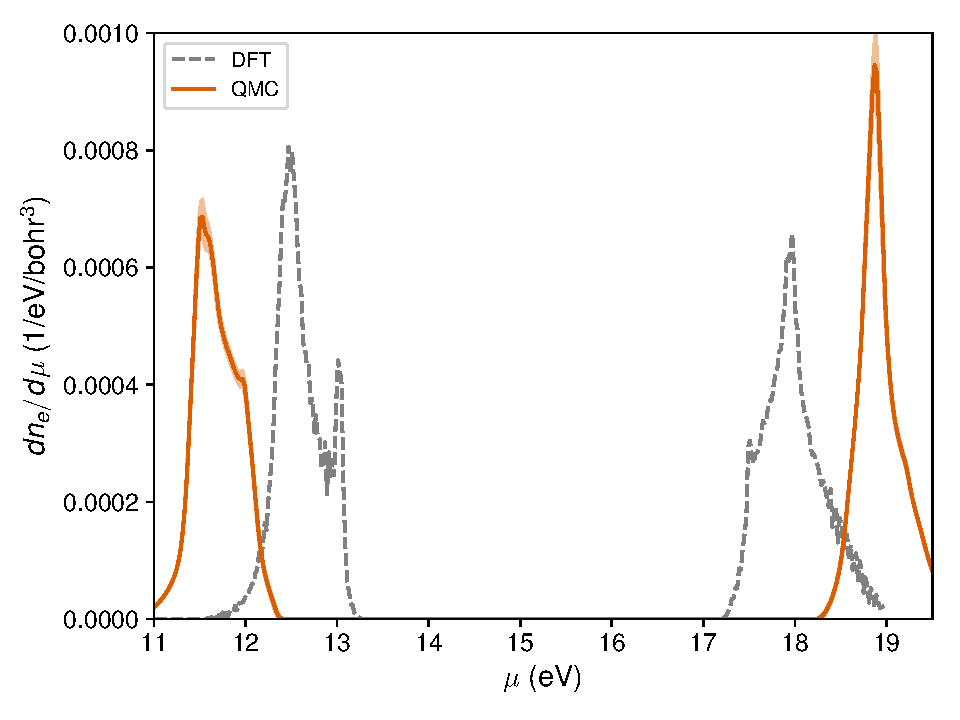
\includegraphics[width=\linewidth]{si35f_nf-c-dndmu}
(a) carbon
\end{minipage}
\begin{minipage}{0.49\columnwidth}
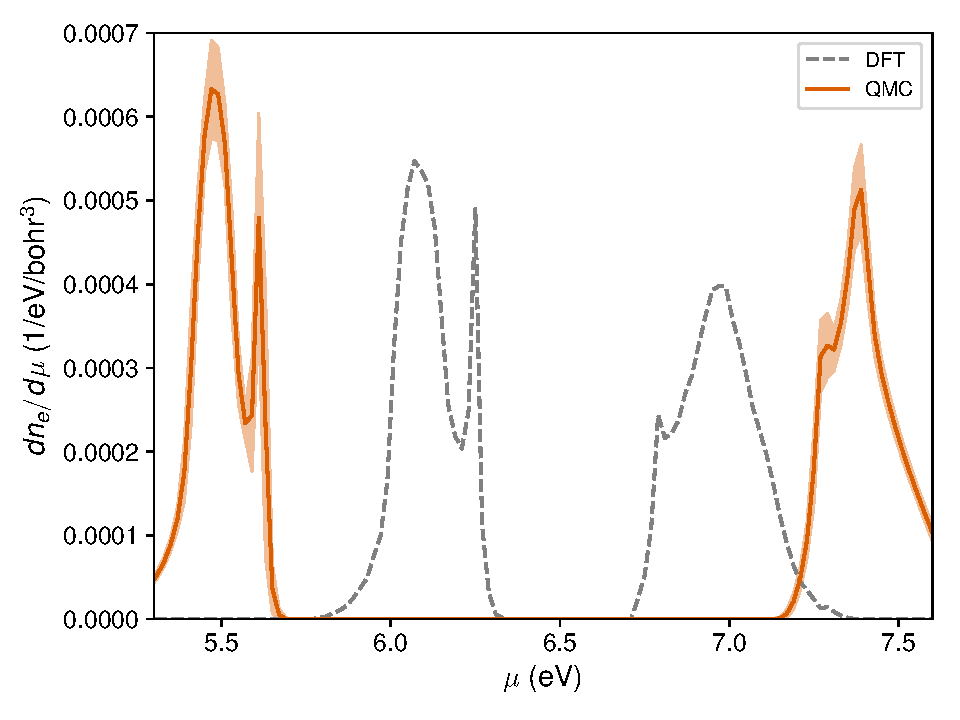
\includegraphics[width=\linewidth]{si35f_nf-si-dndmu}
(a) silicon
\end{minipage}
\caption{Density of states for carbon and silicon near the band edge. Each plot shows the derivative of the  mean electron density with respect to the chemical potential. This is the electronic density of states (DOS) in DFT, so the gap appears as a depleted region. %The shaded regions mark one standard deviation of bootstrap samples. 
The calculated DOS is only valid near the band edge because only the two bands closest to the gap are considered within DFT and QMC. The DFT bands (done in a primitive cell) have been folded into the Brillouin zone (BZ) of the 64-atom supercell to allow comparison with QMC. \label{fig:band_edges}}
\end{figure*}

\begin{table}
\centering
\caption{Energy gaps obtained from GCTAB QMC in eV. The bare gap,
$\Delta_{N}$, was calculated from Eq.~(\ref{gap})
for a finite supercell containing $N$ atoms.
The leading-order finite-size corrections are given by the
screened Madelung constants $|v_M|/\epsilon$, the next-to-leading order by the twist correction of two particle density correlations, $\delta \Delta_s$.
We used the experimental value of $\epsilon$ for C and Si ($5.7$ and $11.7$, respectively) and the value 18.8 for H$_2$ extracted from S(k).
Finite-size corrections were also applied to the band edges,  $\mu^{\pm}$.
The estimate of the gap in the thermodynamic limit is
 $\Delta_\infty=\Delta_{N_e}+|v_M|/\epsilon+\delta \Delta_s$.
From our LDA analysis, we estimate a systematic bias of $\sim 0.1$ eV from the finite twist grid. This bias is larger than the statistical error. SJ indicates Slater-Jastrow trial wave function,
while BF indicates backflow. The lattice constants of carbon and silicon are 3.567 $\text{\AA}$ and 5.43 $\text{\AA}$, respectively. \label{tab:dmc-gcta-gap}}
% C, Si data from si35f/plot.py and si35f/nodvs/read.py
% BF data from si45e/c_interp.py and si45e/plot/dedn.py
\begin{tabular}{lrrrrrrrr}
\hline\hline
 &$r_s$& $N$ & $\Delta_{N}$ & $|v_M|/\epsilon$ & $\delta \Delta_s$ & $\mu^-_{\infty}$ & $\mu^+_{\infty}$ & $\Delta_\infty$ \\
\hline
H$_2$ (BF) & 1.38  &  96 & 3.3(1)   & 0.40 & 0.020 & 6.9(1) & 10.7(1) & 3.8(1) \\
       & 1.34  &  96 & 2.4(1)   & 0.20 & 0.018 & 8.6(1) & 11.2(1) & 2.6(1) \\
\hline
C (BF) & 1.318 &   8 & 3.9(1) & 2.01 & 0.69 & 11.5(1) & 18.1(1) & 6.6(1) \\
\hline
C (SJ) & 1.318 &   8 & 4.0(1) & 2.01 & 0.69 & 11.5(1) & 18.2(1) & 6.7(1) \\
  &  &  64 & 5.8(1)   & 1.00 & 0.02 & 11.9(1) & 18.7(1) & 6.8(1) \\
\hline
Si (BF) & 2.005 &   8 & 0.6(1) & 0.64 & 0.55 & 5.2(1) & 6.9(1) & 1.7(1) \\
\hline
Si (SJ) & 2.005 &   8 & 0.6(1) & 0.64 & 0.58 &  5.2(1) &  7.0(1) & 1.9(1) \\
 &  &  64 & 1.4(1)   & 0.32 & 0.08 &  5.5(1) &  7.3(1) & 1.8(1) \\
 &  & 216 & 1.6(1)   & 0.21 & 0.01 &  5.6(1) &  7.4(1) & 1.8(1) \\
\hline
\hline
\end{tabular}
\end{table}

We have also computed the band gap of solid hydrogen using GCTABC in BF-RQMC calculations
for one of the possible
molecular structures predicted for phase III: C2/c-24 at $r_s = 1.38$ and $r_s=1.34$ (roughly corresponding  to pressures of 234 and 285 GPa, respectively). The results, in Table~\ref{tab:dmc-gcta-gap}, show that the gap and size effects decrease with increasing pressure.
For these calculations, we use calculations for one supercell and use its structure factor to estimate the dielectric constant. From Fig. \ref{fig:H_C2CP250}, we see that HSE DFT slightly underestimates the gap; however, the deviations from the plateau on both sides are quite similar.

\section{Comparison with experiment}
\label{sec:bg-compare}

Our best values for the fundamental electronic gap (BF-DMC)  significantly overestimate the experimentally measured values for C and Si  by 1.1 and 0.5 eV, respectively as shown in Table \ref{tab:c-si-gap-corr}. There are two main sources of systematic errors which need to be taken into account: the use of pseudo-potentials and the neglect of electron-phonon coupling.

The QMC values for C and Si presented above are based on pseudo-potentials to replace the 
core electrons of the atoms. Pseudo-potentials are usually designed for accurate prediction of
static structural quantities. Excitation spectra, in particular, the single-particle excitation gap,
may be less well described.
This has been found in many-body perturbation theory calculations within the $GW$ framework
where all-electron calculations have been shown to lower the gap of C and Si by $\sim -0.3$ eV
\cite{Wu02,GomezAbal08}
with respect to  pseudo-potentials calculations.
Although the actual pseudo-potentials of our QMC simulations differ from those used in the
$GW$ calculations, 
we expect that our QMC values will be shifted by a similar amount; we can roughly transfer
the all-electron correction of $GW$ to our QMC results.

For lighter atoms, electron-phonon coupling leads to a further reduction of the
gap values, even at zero temperature, due to the presence of zero point motion of the ions in
the crystal. For C, $GW$ predicts a significant lowering of the gap by $-0.6$ eV \cite{Giustino10}, whereas a smaller shift between $-60$ meV \cite{Monserrat14} and $-0.1$ eV \cite{Lautenschlager85} is expected from DFT for Si. The effect of thermal expansion is to lower the gap by about 0.01 eV at room temperature for both carbon~\cite{Monserrat2014,Clark1963} and silicon~\cite{Monserrat2016,Logothetidis1986}, beyond the resolution of present calculations.

Considering both, the bias due to the pseudo-potential approximation and the neglect of 
electron-phonon coupling, our BF-DMC calculations for C and Si overestimate the gap by $\sim 0.1-0.2$ eV
(see Table~\ref{tab:c-si-gap-corr}),
larger than our statistical uncertainty. This remaining offset to experiment may
either be due to residual bias of the
fixed-node approximation, or due to effects in pseudo-potential and
e-ph coupling beyond our simple estimations based on $GW$ and DFT.
They could be addressed by more accurate calculations in the future.

For hydrogen, we do not compare to experiment since electron-phonon coupling is
expected to be very large, and the experimental results are not precise.
If we do not make  size corrections, our results are comparable to the Slater-Jastrow DMC calculations of Ref.~\cite{Azadi2017}
where the DFT band structure was corrected by a ``scissor operator'' based on QMC runs at the $\Gamma$ point of the supercell. However, no size effects were observed within the statistical
error in Ref.~\cite{Azadi2017}, so their extrapolated results differ from ours
by $0.3-0.8$ eV (3.0 and 2.3 eV for 250 and 300 GPa).
Comparison to $GW$ values are also
not conclusive: 
Whereas Ref.~\cite{Lebegue2012} provides smaller values of the gaps (1.8 and 1.0 eV for 250 and 300 GPa), the results  of Ref. \cite{McMinis2015} (3.7 and 2.8 eV for 250 and 313 GPa)  are close to our predictions.
However, we note that  the $GW$ calculations were done with
slightly different crystal structures.
In Ref.~\cite{Lebegue2012}, the PBE functional was used to optimize the lattice structure
in contrast to the vdW-DF1 functional of Ref.~\cite{McMinis2015}, shown to be the most accurate functional at this density \cite{Clay2014}. The smaller gap can then
be seen as a consequence of  a larger bond length as it was shown that structures optimized with PBE functional have a larger bond length than the ones with vdW-DF1 \cite{McMinis2015}.
We have recently completed a more detailed analysis of the band gap of molecular hydrogen~\cite{Gorelov2019} using the method introduced here. This discusses extension to disorder coming from nuclear quantum and thermal effects.

\begin{table}
\centering
\caption{Extrapolated band gap
of Si and C from backflow DMC calculations, $\Delta_{BF}$
compared to the experimental values (exp).
We tabulated two main corrections:
the difference  between the gap of an all-electron (AE) and the pseudo-potential (PP)
calculation within GW calculations, and
the neglect of electron-phonon coupling (e-ph).
% with the zero point motion of the ions in the crystal.
%Estimations for both effects from DFT and many-body perturbation theory ($G_0W_0$ or $GW$) 
% indicates that both effects decrease the value of the gap bringing our DMC values closer
%to the experimental ones.
\label{tab:c-si-gap-corr}}
\begin{tabular}{lllll}
\hline\hline
& $\Delta_{BF}$ & AE - PP & e-ph  & exp \\
\hline
C & 6.6(2) &   $-0.26$ ($G_0W_0$) \cite{GomezAbal08} & $-0.6$ ($GW$)~~\cite{Giustino10} & $5.48$ \cite{exp}\\
\hline \\
Si &  1.7(1)  & $-0.25$ ($G_0W_0$)\cite{GomezAbal08}  & $-0.06$ ($DFT$) \cite{Monserrat14} & $1.17$ \cite{exp} \\
 %&    &  & $-0.1$ ($DFT$) \cite{Lautenschlager85} & \\
\hline\hline
\end{tabular}
\end{table}


\section{Conclusions}
\label{sec:bg-conclude}

We have introduced a method to calculate the fundamental gap of insulators and semi-conductors
using QMC. Using grand-canonical twist averaging, 
the value of the gap can be determined at any point in the Brillouin zone whether the system has a direct or indirect gap. Although it is 
possible to map out the whole band structure, we have focused on the minimal, fundamental gap
in this work. We have shown that for charged systems, finite size supercell calculations
are necessarily biased by a finite size error decaying as $1/L$, where the prefactor
is determined by the absolute value of the Madelung constant and the inverse dielectric constant.
We have pointed out that the $1/L$ functional form is encoded in the long wavelength behavior of
the finite size structure factor extrapolating to a non-vanishing value at the origin.
Next-to-leading order effects can be corrected by proper use of twist-averaging in the
two-particle part of the static Coulomb potential. 

We have applied this procedure to determine the fundamental gap of molecular hydrogen at high pressure
and carbon and silicon in the diamond structure at zero pressure. Our finite-size corrected gap values for carbon and silicon are larger than the experimental
ones. We have argued that the bias may be due to the pseudo-potential approximation and the neglect of electron-phonon coupling.

We note that this procedure is not restricted to QMC calculations, but can be applied
within any method which calculates the many-body wave functions and ground-state energies,
e.g., for coupled cluster methods~\cite{Gruber18}. Our results for C and Si demonstrate that
the bias due to the finite size supercell can be corrected for, so
precise values in the thermodynamic limit can be obtained for small supercells
without need for numerical extrapolation.

The procedure here has been developed for perfect crystals but can be generalized 
to systems with disorder, either due to thermal or quantum effects. Furthermore, the procedure provides a starting point 
to address optical, i. e.,  charge neutral excitations. Although neutral excitations are expected to be less sensitive to finite-size effects,
recent calculations \cite{Hunt,Frank19} have observed the same slow $1/L$ decay for the 
optical gap. Since it is often not practical to perform calculations for more than two significantly different supercell sizes, our method suggests that 
the asymptotic behavior of the structure factor provides
the needed insight to whether $1/L$ or $1/L^3$ should be used as a functional form for the
size extrapolation.